\documentclass{article}
\usepackage{graphicx}
\graphicspath{./diagrams}
\usepackage{mathtools}
\usepackage{amsfonts}
\usepackage{amssymb}
\usepackage{amsmath}
\usepackage{amsthm}
\usepackage{physics}
\usepackage{pgfplots}
\pgfplotsset{compat=1.18}

\newtheorem{definition}{Definition}[section]

\title{An Introduction to Complex Numbers}
\author{Joshua John Lee Shi Kai}

\begin{document}
\maketitle
\tableofcontents

\newpage
\section{Introduction}
Complex Analysis is quite similar to real analysis, except it works with complex numbers of the form
$x + iy$, where $x, y \in \mathbb{R}, i^2 = -1$. We represent real numbers on a line, we represent complex
numbers as elements on a plane.

\noindent \\ For example:
\begin{center}
	\begin{tikzpicture}
		\begin{axis}[xmin=0,xmax=3,ymin=0,ymax=3,xlabel = $x$, ylabel = $i$, axis lines = middle]
			\fill (2,1) circle[radius = 2pt] node[above right]{$(2,1)$};
		\end{axis}

	\end{tikzpicture}

\end{center}

\noindent A lot of complex analysis is really similar to real analysis, we can do the usual $+, -, \times, /$,
exponentials, trignometric functions, differentiation, integration. Many of the rules for real analysis work for
complex analysis. $\lim$, series and so on...

\subsection{Some Differences}
\subsubsection{Euler: $e^{ix} = cosx + isinx$}
Trigonometric functions and exponential functions turn out to be almost the same.
Using this we can write all trignometric functions in terms of exponential functions for example,
$cosx = \frac{e^{ix} + e^{-ix}}{2}$. This saves a lot of labour because all the complicated identities
for trigonometric functions are just special cases of identities of exponential functions. So there's a lot
less to remember.
\subsubsection{Differentiability}
For the reals, some functions we can differentiate it once and twice, but not three times. But for a
complex function $\mathbb{C} \rightarrow \mathbb{C}$, once it is differentiable once, it is automatically
differentiable any number of times.
\subsubsection{Integration}
Suppose we want to integrate
\begin{displaymath}
	\int_{0}^{1}f(x)dx
\end{displaymath}
Suppose we want to integrate for real numbers, and there's only one way to go from 0 to 1.
\begin{center}
	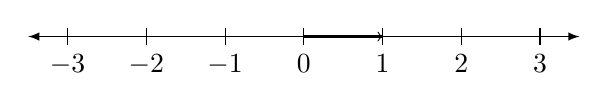
\begin{tikzpicture}
		\draw[latex-latex] (-3.5,0) -- (3.5,0) ; %edit here for the axis
		\foreach \x in  {-3,-2,-1,0,1,2,3} % edit here for the vertical lines
		\draw[shift={(\x,0)},color=black] (0pt,3pt) -- (0pt,-3pt);
		\foreach \x in {-3,-2,-1,0,1,2,3} % edit here for the numbers
		\draw[shift={(\x,0)},color=black] (0pt,0pt) -- (0pt,-3pt) node[below]
		{$\x$};
		\draw[->] (0,0) -- (1.0,0);
		\draw[very thick] (0,0) -- (1,0);
	\end{tikzpicture}
\end{center}
So its quite clear what this integral is meant.

\noindent \\ But if we are integrating in the complex plane,
\begin{center}
	\begin{tikzpicture}
		\begin{axis}[xmin=-1,xmax=3,ymin=-1,ymax=3,xlabel = $x$, ylabel = $i$, axis lines = middle]
			\fill (1,0) circle[radius = 2pt] node[above right]{$(1,0)$};
			\fill (0,1) circle[radius = 2pt] node[above right]{$(0,1)$};
			\addplot [
				domain=0:1,
				samples=150,
				color=blue,
			]
			{2*x - 2*x^2};
			\addplot [
				domain=0:1,
				samples=150,
				color=red,
			]
			{4*x - 4*x^2};
			\addplot [
				domain=0:1,
				samples=150,
				color=purple,
			]
			{-3*x + 3*x^2};

		\end{axis}
	\end{tikzpicture}
\end{center}
There are many ways to go from 0 to 1. So the integral from 0 to 1 seems to depend on which path you take.
Turns out that it almost doesn't. We have Cauch's theorem, that integrals are almost independent of the path
we take from 0 to 1. This turns out to extremely useful. For example in real analysis, there are some equations integrals and sums that we don't learn how to evaluate in ordinary
introductory calculus classes. But you can work out these using complex integration.
\begin{gather*}
	\int_{0}^{\infty}\frac{sinx}{x}dx = \frac{\pi}{2} \\
	\displaystyle\sum_{i=1}^{\infty} \frac{1}{1^2} + \frac{1}{2^2} + \frac{1}{3^2} + \cdots = \frac{\pi^2}{6}
\end{gather*}
\subsection{Analytic Continuation}
Suppose I give you a function from 0 to 1, and ask you to evaluate it at $x = -1$, that would be a
completely stupid question. There's no way to evaluate it at $-1$. There is no real information.
However for complex functions, if I give you a function from 0 to 1, and it is differentiable, it is
automatically determined in any connected region.

\noindent The function on $(a,b)$ is determined uniquely on larger open connected set if it complex differentiable.

\noindent There is a very famous function of this. The Riemann Zeta Function
\begin{displaymath}
	\zeta(s) = \frac{1}{1^s}	+ \frac{1}{2^s}	+ \frac{1}{3^s}	+ \cdots
\end{displaymath}
This is probably the single most notorious function in mathematics, the Riemann hypothesis, which
states that all zeros of $\zeta (s)$ are real or have real part of $\frac{1}{2}$

\begin{center}
	\begin{tikzpicture}
		\begin{axis}[
				legend pos=outer north east,
				title=Riemann Hypothesis,
				xmin=-1, xmax=3,
				ymin=-1, ymax=3,
				axis lines=middle,
				xlabel = $x$,
				ylabel = $i$,
				variable = x,
				trig format plots = rad,
			]

			\draw[purple, thick] (0.5, 3) -- (0.5, -1) node[left, pos=0.6] {$x=\frac{1}{2}$};
			\draw[blue, thick] (1, 3) -- (1, -1) node[right, pos=0.5] {$x=1$};
		\end{axis}
	\end{tikzpicture}
\end{center}
Well the Riemann Hypothesis makes no sense at all because if we try to evaluate it it only converges if
$\Re(s) > 1$
\begin{equation}
	1 + \frac{1}{2} + \frac{1}{3} + \cdots = \infty
\end{equation}
And the function only converges on the right side of $x = 1$. Well it turns out the Riemann Zeta
function can be analytically continued. In other words, there's only one differentiable complex function
that extends the Riemann Zeta function to the whole complex plane, except well, 1 because it would not
converge. Why should people care about the Riemann Zeta function? Well it seems to control prime numbers,
if we draw prime numbers on a real line,
\begin{center}
	\begin{tikzpicture}
		\draw[latex-latex] (0,0) -- (8,0) ; %edit here for the axis
		\foreach \x in  {2,3,5,7} % edit here for the vertical lines
		\draw[shift={(\x,0)},color=black] (0pt,3pt) -- (0pt,-3pt);
		\foreach \x in {2,3,5,7} % edit here for the numbers
		\draw[shift={(\x,0)},color=black] (0pt,0pt) -- (0pt,-3pt) node[below]
		{$\x$};
	\end{tikzpicture}
\end{center}
You can see that they are more dense in some regions, and in some regions
they are less dense. Something like a sort of compression wave. Riemann
discovered that this waves in the primes happen at very precise frequencies,
and the frequencies turn out to be the imaginary parts of the zeroes of the
zeta function. The amplitude of each wave turn out to be the real part. So
the Riemann Hypothesis seems to suggest that primes have a lot of waves going
through them. And all these waves in some sense have the same loudness, or volume.

\subsection{Complex Dynamics}
This is related to a planar set called the Mandel Brot set. We can ask what is the Mandel Brot set?

\noindent You take a complex number, you keep on applying the transformation, while c is fixed
\begin{center}
	\begin{tabular}{lll}
		$z$   & $\rightarrow z^{2} + c$  &                      \\
		$0$   & $\rightarrow 0^{2} + c $ & $\rightarrow \cdots$ \\
		$z_0$ & $\rightarrow z_1$        & $\rightarrow z_2$    \\
		      & $= z_0^2 + c$            & = $z_1^2 + c$        \\
	\end{tabular}
\end{center}
And you can ask whether this sequence is \textbf{bounded}. And this obviously depends on c.
So if this sequence is bounded, it is the same as saying c is in the Mandel Brot set. The thing is
that the Mandel Brot set is incredibly intricate.
\begin{center}
	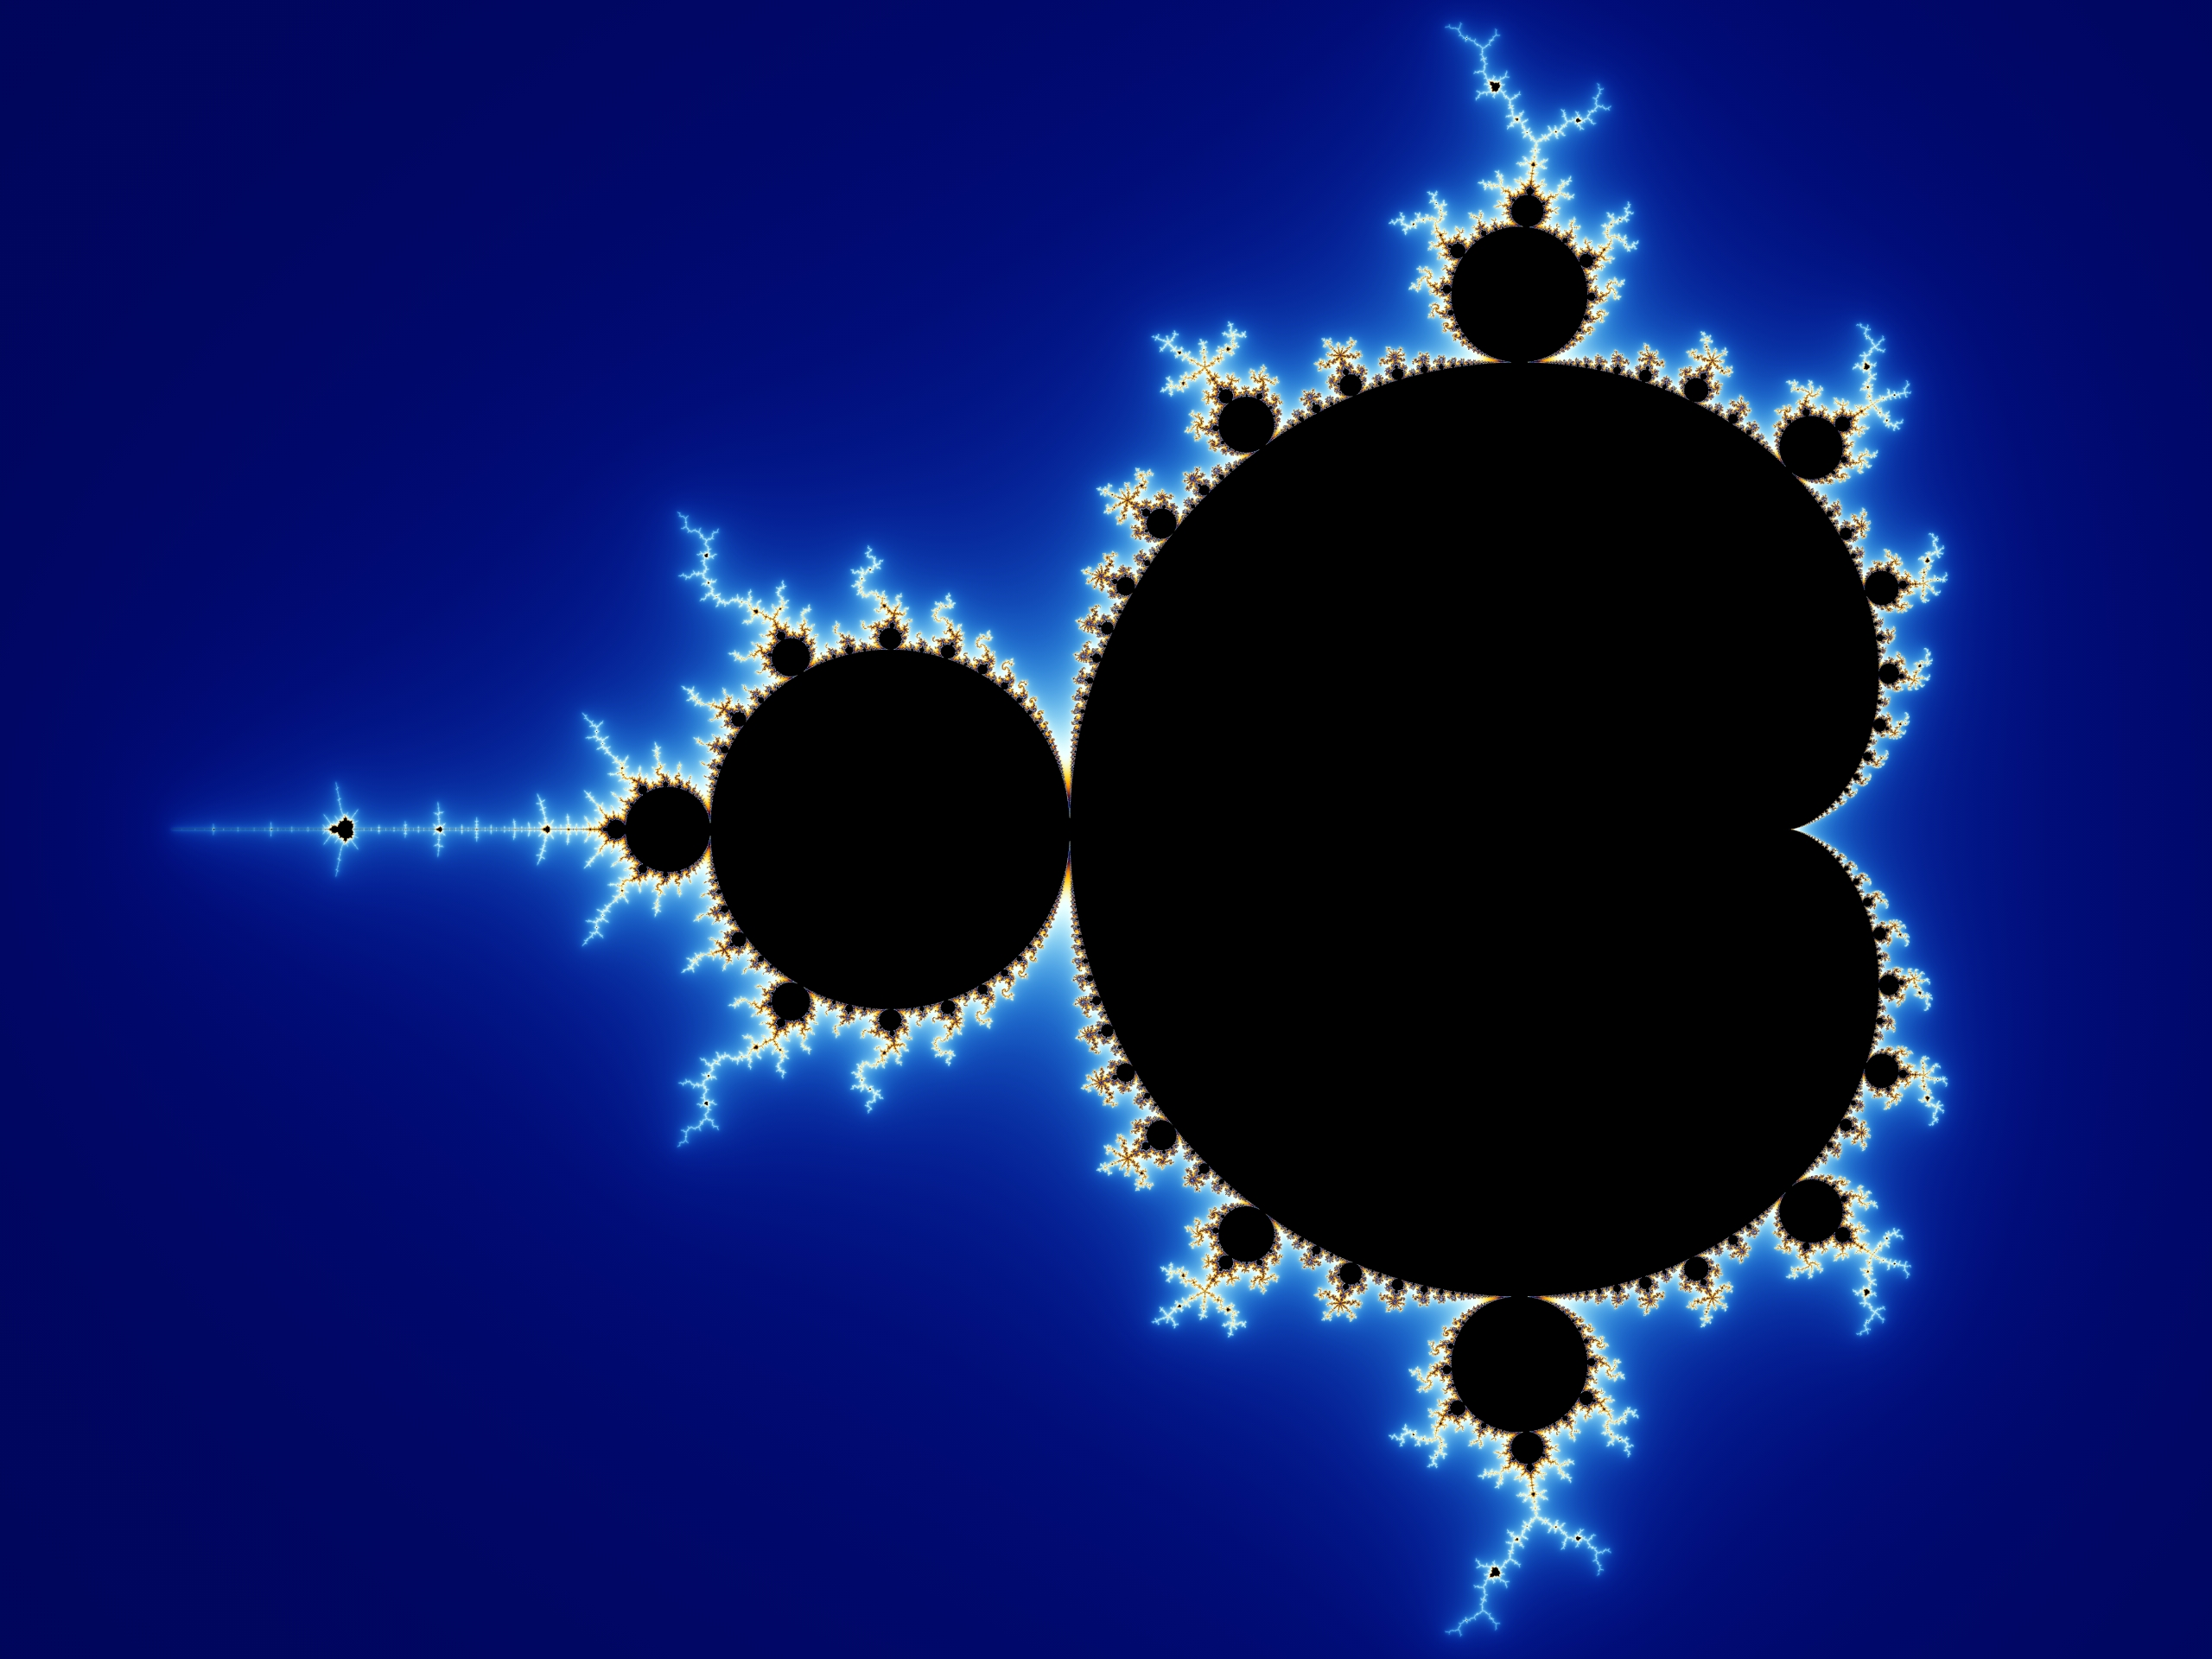
\includegraphics[width=\textwidth]{/diagrams/mandelbrot}
\end{center}

\noindent \\ Well that's the end of the summary.

\section{Complex Arithmetic}
Well if you were a computer, a complex number is nothing more than an ordered pair of numbers $(x,y)$. But
if you were human you would write it as $x + iy$. But as a human, writing it as an ordered pair
is good too because you could understand it as a plane. So you could represent each complex number
as a point in a plane.
\begin{definition}[Addition]
	\begin{displaymath}
		(a + ib) + (c+id) = a+c+ib+id
	\end{displaymath}
\end{definition}
\begin{definition}[Multiplication]
	\begin{align*}
		(a,b)  \cdot (c,d)  & = (ac-bd, ad+bc)             \\
		(a + ib) (c + id)   & = ac + i^{2}bd + ibc + iad   \\
		\text{Since } i^{2} & = -1,                        \\
		                    & \Rightarrow ac-bd + i(bc+ad)
	\end{align*}
\end{definition}
\noindent That's why we remember complex numbers as $x+iy$ form, because
it makes multiplication trivial to remember.
\subsection{The usual stuff}
Does it satisfy the usual rules:
\begin{equation*}
	a(b+c) = ab+ac
	(ab)c = a(bc)
	\cdots
\end{equation*}
Well we could
\begin{enumerate}
	\item Do a long check which we won't do because its long and tedious
	\item Go to an abstract algebra course, and show that the definition of the complex numbers gives a ring
	      with all the usual stuff
\end{enumerate}
\subsection{Division}
Does $a+ib$ has an \textit{inverse} if it is $\neq 0$.

\subsubsection{Complex Conjugation}
Denoted by:
\begin{gather*}
	x + iy \rightarrow x - iy = \overline{x+iy}
\end{gather*}
The reason this turns up a lot is we said $i^{2} = -1$ but $-1$
actually has 2 squareroots because $(-i)^{2} = -1$. So when we talk about
a squareroot of $-1$ we don't really know which squareroot they
are talking about and turns out, they are completely equivalent. Anything
you can say about 1 squareroot you can say about the other squareroot.
So you can sort of flip them around without changing anything. Complex
conjugation actually \textit{preserves} all properties of the complex
numbers. For example:
\begin{gather*}
	\overline{z_{1}z_{2}} = \overline{z_1} \cdot \overline{z_2} \\
	\overline{z_{1}+z_{2}} = \overline{z_1} + \overline{z_2}
\end{gather*}
In fact, complex conjugation $z \rightarrow \overline{z}$ is an \textit{AUTOMORPHISM}
of the complex numbers, $\mathbb{C}$. If you've done a Galois Theory course, another way
of saying is this is the Galois group of the $\mathbb{C}/\mathbb{R}$ is
$\{1,\text{Complex Conjugation}\}$.

\noindent \\ So using complex conjugation, we can find the inverse of any
complex number as follows
\begin{align*}
	z              & = x+iy                                           \\
	z \overline{z} & = (x+iy)(x-iy)                                   \\
	               & = x^{2}+y^{2}                                    \\
	\frac{1 }{z }  & = \frac{\overline{z}}{z\overline{z}}             \\
	\frac{1}{x+iy} & = \frac{x-iy}{(x+iy)(x-iy)}                      \\
	               & = \frac{x-iy}{x^{2}+y^{2}}                       \\
	               & = \frac{x}{x^{2}+y^{2}} - i\frac{y}{x^{2}+y^{2}}
\end{align*}
What you should remember is to multiply the denominator by its complex conjugate. Division by complex
numbers is also reasonably easy.

\subsubsection{Absolute Value}
The absolute distance of $x$ from 0 is $x$ if $x>0$ and $-x$ if $(x<0)$. Similarly, for any complex
number $z$,
\begin{align*}
	z   & = x+iy                 \\
	|z| & = \sqrt{x^{2}+y^{2}}   \\
	    & = \sqrt{z\overline{z}}
\end{align*}
From this, then the following also follows,
\begin{gather*}
	|z_{1}z_{2}| = |z_{1}||z_{2}|
\end{gather*}
All the rules of absolute value also applies,
\begin{gather*}
	|z_{1}-z_{2}| \leq |z_{1}| + |z_{2}|
\end{gather*}
\subsubsection{Application for Complex Arithmetic}
Which integers are sums of 2 squares? Well we know that they are
closed under multiplication. Meaning that if two integers are the sum of two squares then so is
their product.
\begin{proof}
	Let's say we have two integers that are the some of two squares, then
	\begin{displaymath}
		(a^2+b^2)(c^2+d^2) = (ac-bd)^2 + (ad+bc)^2
	\end{displaymath}
	Well where on earth did this come from? It comes from complex numbers!
	We notice that
	\begin{align*}
		a^2+b^2            & = |a+ib|^2              \\
		c^2+d^2            & = |c+id|^2              \\
		(a^2+b^2)(c^2+d^2) & = |(a+ib)(c+id)|^2      \\
		                   & = |ac-bd + i(ad+bc)|^2  \\
		                   & = (ac-bd)^2 + (ad+bc)^2
	\end{align*}
\end{proof}
\noindent The proof with reals doesn't really explain why it exists, it is explained with
complex numbers.
\begin{proof}
	Let's give an example of this
	\begin{align*}
		5           & = 1^2 + 2^2     \\
		13          & = 2^2 + 3^2     \\
		5 \times 13 & = 65            \\
		            & = 8^{2} + 1^{2} \\
		            & = 4^{2} + 7^{2}
	\end{align*}
	So why are there two ways to write 65 as a sum of two squares?
	\begin{align*}
		1^{2} + 2^{2} & = |1+2i|^2 \\
		2^2 + 3^2     & = |2+3i|^2 \\
		(1+2i)(2+3i)  & = -4 + 7i  \\
	\end{align*}
	And you get the first solution, which is actually $(-4)^2 + 7^2$. There's another thing you can do
	which is change one of them to their complex conjugate
	\begin{align*}
		(1+2i)(2-3i) & = 8 + i \\
	\end{align*}
	And there are other things we could do like use the conjugate for the other complex number but it
	will just give variations of the two solutions. So we see that the two ways of writing 65 as a sum
	of two squares correspond to the two different products of complex numbers.
\end{proof}
Next application, let's take a look at pythogoras' theorem, $a^2+b^2=c^2$. And we want to find solutions
to this equation. How can we generate many solutions to this easily?
\begin{align*}
	(a+ib) & = (x+iy)^2     \\
	|a+ib| & = a^2 +b^2     \\
	       & = |(x+iy)^2|^2 \\
	       & = (x^2+y^2)^2  \\
\end{align*}
So now we can just sort of pick any random complex number for $x$ and $y$,
\begin{align*}
	x + iy       & = 2+i                    \\
	(x+iy)^2     & = (2+i)^2                \\
	             & = 3+4i                   \\
	             & = a+ib                   \\
	|a+ib|^2     & = a^2+b^2                \\
	             & = 3^2+4^2                \\
	|(x+iy)^2|^2 & = (|(x+iy)|^2)^2         \\
	             & = ((\sqrt{2^2+1^2})^2)^2 \\
	             & = 5^2
\end{align*}
\subsubsection{Hamilton Quaternions}
Quaternions means a collection of 4 things. so a quarternion is simply
\begin{gather*}
	a + bi + cj + dk \\
	i^2 = -1\\
	j^2 =-1 \\
	k^2 = -1 \\
	ij = k = -ji \\
	jk = i = -kj \\
	ki = j = -ik \\
\end{gather*}
Quaternions are not commutative! But they do behave very similarly to complex numbers. For example,
\begin{align*}
	z                           & = a + bi + cj + dk      \\
	\overline{a + bi + cj + dk} & = a-bi-cj-dk            \\
	z\overline{z}               & = a^2 + b^2 + c^2 + d^2
\end{align*}
So now we can work out the inverse of the quarternion,
\begin{gather*}
	\frac{1}{a+bi+cj+dk} = \frac{a-bi-cj-dk}{a^2+b^2+c^2+d^2} \\
\end{gather*}
You realise that if the quarternion is non-zero, then the denominator would be non-zero, so all
non-zero quarternions have inverses.
\section{Roots}
Do Complex Numbers have square roots?
Can we find
\begin{gather*}
	\sqrt{2+i} \\
	\sqrt[3]{2+i} \\
	\cdots
\end{gather*}
The answer is YES! To understand this, we have to understand the geometric meaning of multiplication.
To do this, we express multiplication in terms of polar coordinates.

\begin{center}
	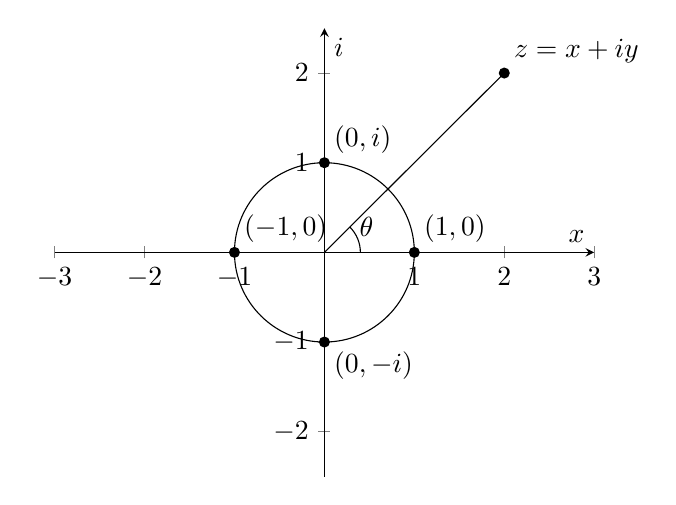
\begin{tikzpicture}
		\begin{axis}[
				clip=false,
				legend pos=outer north east,
				title=,
				xmin=-3, xmax=3,
				ymin=-2.5, ymax=2.5,
				axis lines=middle,
				xlabel = $x$,
				ylabel = $i$,
				variable = x,
				trig format plots = rad,
			]
			\draw (axis cs: 0, 0) circle [radius=1];
			\fill (1,0) circle[radius = 2pt] node[above right]{$(1,0)$};
			\fill (0,1) circle[radius = 2pt] node[above right]{$(0,i)$};
			\fill (0,-1) circle[radius = 2pt] node[below right]{$(0,-i)$};
			\fill (-1,0) circle[radius = 2pt] node[above right]{$(-1,0)$};
			\fill (2,2) circle[radius = 2pt] node[above right]{$z=x+iy$};
			\draw (0,0)--(2,2);
			\draw (0.4,0) arc (0:45:0.4) node[right]{$\theta$};
		\end{axis}
	\end{tikzpicture}
\end{center}
We have the usual way to go about changing from cartesian to
polar coordinates.
\begin{gather*}
	r = |z| \\
	tan\theta = \frac{y}{x}\\
	x = rcos\theta \\
	y = rsin\theta \\
\end{gather*}
Now you notice if we take the values of absolute value one (the circle),
these actually form a group. A \textbf{group} is a set that is closed under
multiplication and inverses. For example,
\begin{gather*}
	|z_1| = 1 \\
	|z_2| = 1 \\
	|z_1 z_2| = 1 \\
	|z^{-1}| = 1 \\
\end{gather*}
So we can multiply and divide points on the circle group. We also see that
any complex number $z$, can be written as a point on the circle group,
times a positive real number.
\begin{align*}
	\text{Point on the circle group: } & cos\theta + isin\theta               \\
	\text{Any Complex Number: }        & z = r \cdot (cos\theta + isin\theta)
\end{align*}
Every non-zero complex number $z$, can be written \textit{uniquely} as
$z = a \cdot b$ where $a$ is a positive real, and $b$ is in the circle group ($|b| = 1$).
Another way of writing this is $\mathbb{C}^{x} \coloneqq \mathbb{R}_{>0} \times \mathbb{S}^{1}$, where
$\mathbb{C}^{x}$ means take the complex numbers under multiplication and throw away the zero, positive
reals, and the circle group where $\mathbb{S}$ means sphere and the superscript means it is one-dimension.

\subsection{Multiplication in $S^1$}
There are two ways to do multiplication in $S^1$, namely,
\begin{enumerate}
	\item Mutiply them as complex numbers.
	\item Multiply them by adding angles.
\end{enumerate}
And we want to show that they are the same.
\begin{proof}
	Complex multiplication:
	\begin{gather*}
		(cos\theta_1+isin\theta_1) \times (cos\theta_2+isin\theta_2) \\
		= cos\theta_1 cos\theta_2 - sin\theta_1 sin\theta_2 + i(cos\theta_1 sin\theta_2 + cos\theta_2 sin\theta_1)
	\end{gather*}
	Similarly for the addition of angles,
	\begin{gather*}
		cos(\theta_1 + \theta_2) = cos\theta_1 cos\theta_2 - sin\theta_1 sin\theta_2 \\
		sin(\theta_1 + \theta_2) = sin\theta_1 cos\theta_2 + cos\theta_1 sin\theta_2
	\end{gather*}
	So multiplying the complex numbers on the circle, is the same as adding their angles.
\end{proof}
\noindent This shows that complex numbers are really good for rotations in $\mathbb{R}^2$. Similarly
quarternions are really good for rotations of $\mathbb{R}^3$ and $\mathbb{R}^4$. Navigation systems
often make use of quarternions to calculate rotations.

\subsubsection{Summary}
To multiply two complex numbers $z_1, z_2$,
\begin{enumerate}
	\item Multiply absolute values
	\item Add angles (argument)
\end{enumerate}
You can multiply complex numbers by just sort of staring at them, not much algebraic stuff needed.

\subsection{Square Roots}
So $\sqrt{z}$ simply has half the argument, $\theta$, and the absolute value $= \sqrt{|z|}$. This sort
of shows that every complex number has a square root. Let's show this graphically.

\begin{center}
	\begin{tikzpicture}
		\begin{axis}[
				clip=false,
				legend pos=outer north east,
				title=,
				xmin=-3, xmax=3,
				ymin=-2.5, ymax=2.5,
				axis lines=middle,
				xlabel = $x$,
				ylabel = $i$,
				variable = x,
				trig format plots = rad,
			]
			\draw (axis cs: 0, 0) circle [radius=1];
			\fill (-1,2) circle[radius = 2pt] node[above right]{$z$};
			\fill (0.78,1.27) circle[radius = 2pt] node[above right]{$\sqrt{z}$};
			\draw (0,0)--(-1,2);
			\draw (0,0)--(0.78,1.27);
			\draw (0.4,0) arc (0:116.56:0.4) node[above]{$\theta$};
			\draw (0.5,0) arc (0:58.28:0.5) node[right]{$\theta/2$};
		\end{axis}
	\end{tikzpicture}
\end{center}
We notice that $\sqrt{z}$ has half the argument of $z$, and the real part
of $\sqrt{z}$ is $\sqrt{|z|}$. So the two square roots of $z$ are
$\sqrt{z}$ and $-\sqrt{z}$.

\subsection{Other Roots}
Just as numbers have more than one square root, they have more than
one 5th root, so if we take $\frac{\theta}{5}$, we can also take $\frac{\theta + 2\pi}{5}$,
$\frac{\theta+4\pi}{5}$ and so on...

\begin{center}
	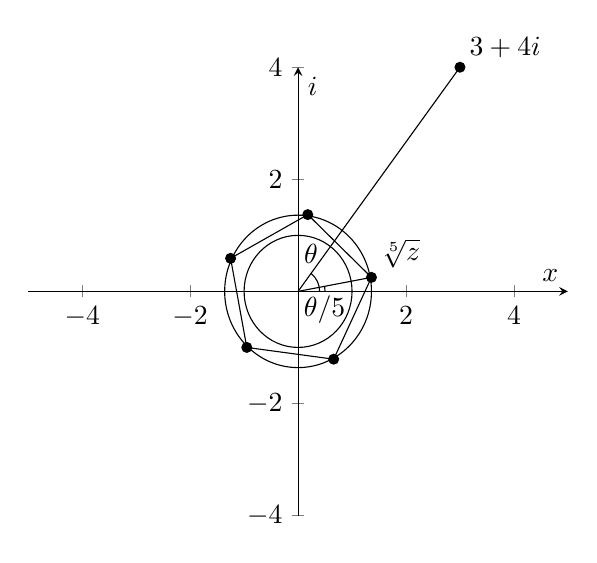
\begin{tikzpicture}
		\begin{axis}[
				clip=false,
				legend pos=outer north east,
				title=,
				xmin=-5, xmax=5,
				ymin=-4, ymax=4,
				axis lines=middle,
				xlabel = $x$,
				ylabel = $i$,
				variable = x,
				trig format plots = rad,
			]
			\draw (axis cs: 0, 0) circle [radius=1];
			\draw (axis cs: 0, 0) circle [radius=1.36];
			\fill (3,4) circle[radius = 2pt] node[above right]{$3+4i$};
			\fill (1.36,0.25) circle[radius = 2pt] node[above right]{$\sqrt[5]{z}$};
			\fill (0.18,1.37) circle[radius = 2pt] node[above right]{};
			\fill (-1.25,0.59) circle[radius = 2pt] node[above right]{};
			\fill (-0.95,-1.0) circle[radius = 2pt] node[above right]{};
			\fill (0.66,-1.21) circle[radius = 2pt] node[above right]{};
			\draw (1.36,0.25)--(0.18,1.37);
			\draw (0.18,1.37)--(-1.25,0.59);
			\draw (-1.25,0.59)--(-0.95,-1.0);
			\draw (-0.95,-1.0)--(0.66,-1.21);
			\draw (0.66,-1.21)--(1.36,0.25);
			\draw (0,0)--(3,4);
			\draw (0,0)--(1.36,0.25);
			\draw (0.4,0) arc (0:53.13:0.4) node[above]{$\theta$};
			\draw (0.5,0) arc (0:10.62:0.5) node[below]{$\theta/5$};
		\end{axis}
	\end{tikzpicture}
\end{center}
The five roots lie on a regular pentagon. And the same happens if you take
any nth roots of any non-zero complex number, you find that there are going to be
n roots, and they lie on the vertices of a nice regular, n-sided polygon. And you
can find out these values explicitly by working out the argument and absolute value of z.

\noindent \\ So any complex number, $z$, has an n-th root. If $z$ is non-zero, it is going to have
n distinct, n-th roots. So polynomials of the form $z^{n} - a$ always has root. The same happens
for more complex polynomials, and will be shown later to always have a complex root. We sometimes
express this by saying that $\mathbb{C}$ is algebraically closed. "algebraically closed" just means
that whenever you have any non constant polynomial, you can always find a root of that polynomial.

\subsection{Multiple Angle Formulas}
Everyone is familiar with the old trusty angle formulas
\begin{gather*}
	cos2\theta = cos^2\theta - sin^2\theta \\
	cos3\theta = cos^3\theta - 3cos\theta sin^2\theta = 4cos^3\theta - 3cos\theta
\end{gather*}
You \textit{could} prove these formulas by doing some tedious algebra, but with complex numbers, the
work becomes a lot less. We get it from the binomial theorem,
\begin{align*}
	cosn\theta + isinn\theta & = (\cos\theta + i\sin\theta)^n                                                                                       \\
	                         & = \binom{n}{0}(\cos\theta)^n + i\binom{n}{1}(cos\theta)^{n-1}\sin\theta - \binom{n}{2}(cos\theta)^{n-2}(sin\theta)^2
\end{align*}
And then just take real parts of both sides.
\begin{gather*}
	\cos n\theta = (\cos\theta)^n - \binom{n}{2} (\cos\theta)^{n-2}(\sin\theta)^2 + \cdots
\end{gather*}
\section{Elementary Transcendental Functions}
This section will discuss $e^x, \log, \sin, \cos, \tan,$ and so on... We will start with the exponential
function, and see that all the others are just special cases of it.
\subsection{Exponential}
We can define the exponential function using the normal power series, as we do for over the reals,
\begin{gather*}
	e^z = 1 + z + \frac{z^2}{2!} + \frac{z^3}{3!} + \cdots
\end{gather*}
So we can ask the question, does this converge? Turns out it is absolutely convergent. And if a series
of complex numbers are absolutely convergent, then so is the series of real parts, and the same for the
imaginary parts.
\begin{align*}
	e^{z_1+z_2}                                    & = e^{z_1}e^{z_2}                                                     \\
	\displaystyle\sum_{n}^{}\frac{(z_1+z_2)^n}{n!} & = \displaystyle\sum_{n,m}^{}\frac{\binom{n}{m}z_1^m z_2^{n-m}}{n!}   \\
	                                               & = \displaystyle\sum_{n,m}^{}\frac{z_1^m}{m!}\frac{z_2^{n-m}}{(n-m)!} \\
	                                               & = \displaystyle\sum_{n,m}^{}\frac{z_1^m}{m!}\frac{z_2^n}{n!}         \\
	                                               & = e^{z_1}e^{z_2}
\end{align*}
You realise we did some rearrangement, but that's fine because everything is absolutely
convergent. So let's try now to calculate it,

\begin{align*}
	z      & = x+iy                                                                                   \\
	e^z    & = e^x e^{iy}                                                                             \\
	e^{iy} & = 1+iy+\frac{i^2y^2}{2!}+\frac{i^3y^3}{3!}+\cdots                                        \\
	       & = 1 + iy - \frac{y^2}{2!}	 - \frac{iy^3}{3!} + \frac{y^4}{4!} + \frac{iy^5}{5!} + \cdots
\end{align*}
We realise that
\begin{gather*}
	1 - \frac{y^2}{2!} + \frac{y^4}{4!} + \cdots  = \cos y \\
	iy - \frac{iy^3}{3!} + \frac{iy^5}{5!} + \cdots = i\sin y
\end{gather*}
This brings us to Euler's identity, where $e^{iy} = \cos y + i\sin y$. Which
allows us to work out the exponential for all complex $z$. Also it
follows that,
\begin{gather*}
	y = \pi \\
	e^{\pi i} = -1 \\
	y = 2 \pi \\
	e^{2\pi i} = 1 \\
	e^{2n\pi i} = 1, \text{ for } n \in \mathbb{Z}
\end{gather*}
We can also say that the exponential function is a homomorphism of groups. We know that
\begin{gather*}
	\exp(z_1 + z_2) = \exp(z_1)\exp(z_2) \\
\end{gather*}
Therefore, we see from algebra courses that this is just a homomorphism from the complex numbers under
addition, to the complex numbers under multplication. $ \mathbb{C} \rightarrow
	\mathbb{C}^\times $. Saying its a homomorphism just says that it turns addition into multiplication.
We also notice that this exponential map is onto. So, provided that $r$ is non-zero,
\begin{gather*}
	r(\cos\theta + i \sin \theta ) = \exp(\log r + i \theta)
\end{gather*}
We can also ask what is the kernel? Where $	\exp(x + iy) = 1$?
\begin{gather*}
	\exp(x+iy) = \exp(x)(\cos y + i \sin y)
\end{gather*}
Thus we can see that $x = 0$, and $y$ has to be some multiple of $2\pi$.

\noindent \\ \textbf{Note:} For the reals, we also get a map from the reals under addition to the
reals under multiplication, $\mathbb{R} \rightarrow \mathbb{R}^\times$. Except this time, there's
no kernel and the map is not unto. It is injective but surjective. Whereas the complex exponentials
is surjective but not injective.
\subsection{Logarithm}
Solve: $e^{a + bi} = z$
\begin{align*}
	z      & = r(\cos\theta + i\sin\theta) \\
	a + bi & = \log z                      \\
	e^a    & = r                           \\
	       & = |z|                         \\
	a      & = \log|z|, z \neq 0           \\
	\theta & = \arg(z)
\end{align*}
The problem is that $arg(z)$ is not unique, so $\theta$ is only defined
up to multiples of $2\pi$. $\log(z)$ NOT unique, only defined up to multiples
of $2\pi i$.

\noindent \\ We can also ask if,
\begin{gather*}
	z_1^{z_2} = \exp(z_2 \log(z_1))
\end{gather*}
Is well defined, since $\log(z_1)$ is ambiguous, there are only 2 cases where this function is well
defined.
\begin{enumerate}
	\item $z_1 > 0$ and REAL, take the real part of $\log(z_1)$
	\item $z_2$ is an integer, $\exp(n\log(z_1)) = \exp(n2\pi i) = 1$
\end{enumerate}
\subsection{Trigonometric Functions}
\begin{gather*}
	e^{iz} = \cos z + i\sin z \\
	e^{-iz} = \cos z - i\sin z \\
	\frac{e^{iz}+e^{-iz}}{2} = \cos z \\
	\frac{e^{iz}-e^{-iz}}{2i} = \sin z
\end{gather*}
An amazing unification of exponential functions and trigonometric functions. In
real analysis, they seem so different. Over the complex numbers, they seem like
almost the same function. All identities of trigonometric functions also follow
from the exponential functions.

\subsection{Applications of Trigonometric Functions}
Suppose you want to solve a simple linear differential equation.
\begin{gather*}
	a \frac{d^2y}{dx^2} + b \frac{dy}{dx} + cy = 0 \\
\end{gather*}
If you've been to a real analysis course, you know you tend to be able to find the solution,
\begin{gather*}
	y = e^\alpha \cos \beta x
\end{gather*}
and its really a bit of a mess checking what $\alpha, \beta$ has to be for this to be a solution.
With complex numbers this becomes a lot easier to solve, you just substitute in $y = e^{\lambda x}$.
\begin{gather*}
	a \lambda^2 e^{\lambda x} + b \lambda e^{\lambda x} + c e^{\lambda x} = 0 \\
	a \lambda^2 + b \lambda + c = 0
\end{gather*}
So now $\lambda$ is given by the root of some quadratic equation. We get a much simpler form for the
solution. As an example,
\begin{gather*}
	\frac{d^2y}{dx^2} + 2 \frac{dy}{dx} + 2y = 0 \\
	\Rightarrow \lambda^2 + 2 \lambda + 2 = 0 \\
	\Rightarrow \lambda = -1 \pm i \\
	y = e^{(1+i)x}, e^{(i-1)x} \\
	\Rightarrow y = e^x \cos x, e^x \sin x
\end{gather*}
Another way complex numbers make things simplier is if you're doing Fourier series. If you have a
function that's periodic,
\begin{gather*}
	f(x) = f(2\pi + x) \\
	\Rightarrow f(x) = \sum_{n > 0}a_n \sin (nx) + \sum_{n \geq 0}b_n \cos (nx)
\end{gather*}
Now if you use complex numbers you can very easily simplify this, because sin and cos can be written
as exponentials.
\begin{gather*}
	f(x) = \sum_{n \in z}c_n e^{inx}
\end{gather*}
This makes computing the fourier series a lot easier and neater.

\section{Complex Derivatives}
We are not going to go straight into complex derivatives, but we are going to look at real derivatives
of complex functions.
\subsection{Real Derivatives of Complex Functions}
Let's take $w = u + iv$ is a function of $z = x + iy$, where $u, v, x, y \in \mathbb{R}$. Such that
$u, v$ are functions of $x,y$. First we need to write $u, v$ as a vector.
\begin{gather*}
	\begin{bmatrix}
		u(x,y) \\
		v(x,y)
	\end{bmatrix}
	=
	\underbrace{
		\begin{bmatrix}
			u(x_0, y_0) \\
			v(x_0, y_0)
		\end{bmatrix}
		+
		\begin{bmatrix}
			a & b \\
			c & d
		\end{bmatrix}
		\begin{bmatrix}
			x - x_0 \\
			y - y_0
		\end{bmatrix}
	}_{\text{linear function}}
	+ \epsilon
\end{gather*}
If you compare it with the real derivative, you see that it is much the same. Except that now we are
doing it with two variables. Again, this error should be less than any linear function such that
\begin{gather*}
	\text{As } (x,y) \rightarrow (x_0,y_0)\\
	\frac{|\epsilon|}{\text{dist}(x,y),(x_0,y_0)} \rightarrow 0
\end{gather*}
Saying that $w$ is differentiable at the point $z_0$ just means that we can approximate the function
$w$ by this linear function with a small error term, $\epsilon$. The matrix,
\begin{gather*}
	\begin{bmatrix}
		a & b \\
		c & d
	\end{bmatrix}
\end{gather*}
can also be written as the partial derivates,
\begin{gather*}
	\begin{bmatrix}
		\frac{\delta u}{\delta x} & \frac{\delta u}{\delta y} \\
		\frac{\delta v}{\delta x} & \frac{\delta v}{\delta y}
	\end{bmatrix}
\end{gather*}
So far we haven't done anything in complex analysis, all we have done is discussed a function from the
real plane to the real plane, and discussed whether its differentiable. What we have defined here
is just real differentiability.
\subsection{Complex Derivatives}
Now we want to define a complex derivative. With the same $w = u + iv$ which is a function of
$z = x + iy$, where $u, v, x, y \in \mathbb{R}$. But now we have to take the complex plane into
account.
\begin{gather*}
	w(z) = w(z_0) + A(z-z_0) + \epsilon
\end{gather*}
Here $A$ is a complex number, and since $(z - z_0)$ is the matrix
$
	\begin{bsmallmatrix}
		x - x_0 \\
		y - y_0
	\end{bsmallmatrix}
$, then A would have to be
$
	\begin{bsmallmatrix}
		\Re(A) & -\Im(A) \\
		\Im(A) & \Re(A)
	\end{bsmallmatrix}
$. This matrix is the representation of:
\begin{gather*}
	A(x + iy) = \Re(A) \cdot x - \Im (A) \cdot y + i (\Im(A)\cdot x + \Re(A) \cdot y)
\end{gather*}
Now if we compare this matrix $A$ with the partial derivates from the real derivates, we see that,
\begin{gather*}
	A =
	\begin{bmatrix}
		\frac{\delta u}{\delta x} & \frac{\delta u}{\delta y} \\
		\frac{\delta v}{\delta x} & \frac{\delta v}{\delta y}
	\end{bmatrix}
	=
	\begin{bsmallmatrix}
		\Re(A) & -\Im(A) \\
		\Im(A) & \Re(A)
	\end{bsmallmatrix}
\end{gather*}
So for $w$ to be differentiable as a complex function, this equality must hold. The \textbf{Cauchy Riemann}
Equations say that the necessary and sufficient condition for any real differentiable function
to be complex differentiable, is as follows
\begin{gather*}
	\frac{\delta u}{\delta x} = \frac{\delta v}{\delta y} \\
	\frac{\delta v}{\delta x} = -\frac{\delta u}{\delta y}
\end{gather*}
We can also express $A$ in terms of a limit,
\begin{gather*}
	A = \lim_{dz \rightarrow 0} \frac{dw}{dz}
\end{gather*}
where,
\begin{gather*}
	dw = w(z) - w(z_0) \\
	dz = z - z_0
\end{gather*}
\subsection{Holomorphic}
Suppose $w$ is a complex function of $z$, where $z \in U$, for some open set $U \in \mathbb{C}$. Then
$w$ is called \textbf{HOLOMORPHIC} if it has a complex derivative everywhere on $U$. You'll sometimes
see the word \textit{analytic} used instead, however this means that it has a power series expansion
that converges at each point. What we will prove later that for complex functions, they are holomorphic
on an open region if and only if they have a convergent power series expansion at every point.

\subsection{Wertinger Derivatives}
We can also define the partial derivatives with respect to $z$ and $\overline{z}$.
\begin{gather*}
	\frac{\delta}{\delta z} = \frac{1}{2}(\frac{\delta}{\delta x} - i\frac{\delta}{\delta y}) \\
	\frac{\delta}{\delta \overline{z}} = \frac{1}{2}(\frac{\delta}{\delta x} + i \frac{\delta}{\delta y})
\end{gather*}
The reason we define it like this is because they give the following results
\begin{gather*}
	\frac{\delta}{\delta z } z = 1 \\
	\frac{\delta}{\delta z } \overline{z} = 0 \\
	\frac{\delta}{\delta \overline{z} } z = 0 \\
	\frac{\delta}{\delta \overline{z} } \overline{z} = 1
\end{gather*}
Which is what we expect from the derivatives of $z$ and $\overline{z}$. So now we can write the
Cauchy Riemann equations,
\begin{gather*}
	\frac{\delta w}{\delta \overline{z}} = 0
	\begin{cases}
		\frac{\delta u}{\delta x} = \frac{\delta v }{\delta y} \\
		\frac{\delta u}{\delta y} = -\frac{\delta v}{\delta x}
	\end{cases}
\end{gather*}
This suggests that holomorphic means depends on $z$ but not $\overline{z}$.
\subsection{Examples Of Holomorphic Functions}
The obvious linear functions,
\begin{gather*}
	1, z
\end{gather*}
For any $f, g$ that are holomorphic on $U \in \mathbb{C}$,
\begin{gather*}
	f+g, f-g, fg, f/g, f(g(z))
\end{gather*}
is also holomorphic, the proof is the same as the one in real analysis.

\noindent \\ For any convergent power series where $|z| < k$ for some constant $k$.
\begin{gather*}
	a_o + a_1 z + a_2 z^2 + \cdots
\end{gather*}
The proof is very similar to the proof in a real analysis. This means that
\begin{gather*}
	\sin, \cos, \tan, \exp, \log
\end{gather*}
are all differentiable. (when they are defined of course)

\noindent \\ If $f$ is holomorphic, then $\frac{df}{dz}$ is also holomorphic. Which is totally false
for real variables.

\subsection{Examples Of Non-Holomorphic Functions}
The following are not holomorphic and can be easily verified by checking the Cauchy Riemann equations.
\begin{gather*}
	\Re(z), \Im(z), |z|, |z|^2 = z\overline{z}, \overline{z}
\end{gather*}

\section{Harmonic Functions}
Given the complex function $w = u + i v$ of a complex variable $z = x + i y$, where $u,v,x,y \in
	\mathbb{R}$ and $w,z \in \mathbb{C}$. Suppose we are given the function $U(x,y)$, can we find a
holomorphic function $w$ so that $u$ is the $\Re(w)$? Following the Cauchy Riemann equations,
\begin{gather*}
	\frac{\delta u}{\delta x} = \frac{\delta v}{\delta y} \\
	\frac{\delta u}{\delta y} = -\frac{\delta v}{\delta x} \\
	\Rightarrow \frac{\delta^2 u}{\delta x^2} = \frac{\delta^2 v}{\delta x \delta y}
	= -\frac{\delta^2 u}{\delta y^2}
\end{gather*}
This presents the non-trivial condition that
\begin{gather*}
	\frac{\delta^2 u}{\delta x^2} + \frac{\delta^2 u}{\delta y^2} = 0
\end{gather*}
This is the most basic of all partial differentiable equations called the Laplace equation. Functions
that satisfy this equation are called harmonic equations. This has a physical interpretation, it gives
you the steady state heat of some planar region, if you fix the temperature on the boundaries, the steady
state of the object would satisfy the Laplace equation. It is also usually written as the Laplace
operator, $\Delta = \frac{\delta^2}{\delta x^2} + \frac{\delta^2}{\delta y^2}$. So the Laplace equation
above just says that $\Delta U = 0$.

\noindent \\ \textbf{Example:} Find all harmonic polynomials in $x,y$. So we want to solve $\Delta f = 0$
where $f$ is just a polynomial. We can just take polynomials in $z$ which are holomorphic, and use
their real and imaginary parts.
\begin{center}
	\begin{tabular}{c | c c c c c}
		$f$      & 1 & $z$ & $z^2$     & $z^3$       & $\cdots$ \\
		$\Re(f)$ & 1 & $x$ & $x^2-y^2$ & $x^3-3xy^2$ & $\cdots$ \\
		$\Im(f)$ & 0 & $y$ & $2xy$     & $3x^2y-y^3$ & $\cdots$ \\
	\end{tabular}
\end{center}
Any linear combination of these polynamials is also harmonic. These form a basis of all harmonic
polynomials. Another example would be to let $z e^z$ be holomorphic, hence,
\begin{gather*}
	z e^z = (x+iy) e^x (\cos y + i \sin y) \\
	\Rightarrow \Re(ze^z) = e^x(x \cos y - y \sin y)
\end{gather*}
Hence we've shown that the real part of any holomorphic function must be harmonic. That might also
ask us to consider, is any harmonic function $u$, the real part of some holomorphic function $w = u
	+ iv$? We will see that it depends on the connected open set $U \subset \mathbb{C}$ on which the
function $u$ lies.

\section{Integration}
In real analysis, we can integrate from $a$ to $b$ some real valued function,
\begin{gather*}
	\int_{a}^{b} f(x) dx
\end{gather*}
if $f$ is continuous. And we want to find something similar for the complex variables. We might
want to define some function $f$,
\begin{gather*}
	\int_{a}^{b} f(z) dz
\end{gather*}
where $a, b, z, \in \mathbb{C}$, and $f$ is holomorphic. The problem being that we can not simply
integrate complex variables as easily as we do with real variables, as they are path dependent. A
more accurate definition of the integral of complex variables would be,
\begin{gather*}
	\int_{C}f(z)dz
\end{gather*}
Where $C$ is a path from $a$ to $b$. Given by the function,
\begin{gather*}
	\rho : \mathbb{R} \rightarrow \mathbb{C}
\end{gather*}
Of which $\rho(r) = a$ and $ \rho(s) = b$ for some $r, s \in \mathbb{R}$. Then if $\rho$ has a continuous
derivative,
\begin{gather*}
	z = p(x) \\
	dz = p'(x)dx \\
	\Rightarrow \int_{C}f(z)dz = \int_r^s f(p(x))p'(x)dx
\end{gather*}
If the path doesn't have a continuous derivative, it is quite common to split the path up to a finite number of
pieces and find out each integral individually and sum them up. Another way to look at it is in its form of vectors.
For some $f = u + iv$ and $z = x + iy$,
\begin{gather*}
	\int_C f(z)dz = \int_C (u + iv) (dx + idy) \\
	= \int_C udx - vdy + i \int_C vdx + udy
\end{gather*}
This integral is almost always independent of parameterization, except for its direction. Other basic properties
of integrals that are very much like real integrals.
\begin{gather*}
	\int_{C_1} f(z)dz + \int_{C_2} f(z)dz = \int_{C_1 \cup C_2} f(z)dz \\
	\int_C (f + g) dz = \int_C f dz + \int_C g dz
\end{gather*}
And a little less obvious property
\begin{gather*}
	|\int_C f(z) dz | \leq M|C|
\end{gather*}
Where $|C|$ is the length of $C$ and $M$ is the upper bound of $|f|$.
\end{document}
